\subsubsection{Membrane Transport}
\index{Winterhalter, Mathias}

\paragraph{Research Team}
%
Mathias Winterhalter (Professor), Yannic Ramaye (Postdoc), Helge
Weingart (Postdoc, Project Manager), Tivadar Mach (PhD Student), Joana
Gomes (PhD Student), Raghavendra Palankar (PhD Student), Que Tien Tran
(PhD Student), Stefanie T�mmers (PhD Student)\\

The outer cell wall of \textit{Escherichia coli} contains a number of channel forming
proteins called porins. Such channels allow e.g. bacteria to harvest nutrients.
Our main research focus is on the characterisation of transport across such
membrane channels. For this our method of choice is to reconstitute
membrane channels into planar lipid bilayers and characterise them by time
resolved ion current. For example, previously we have been able to follow the
translocation of single sugar molecules through Maltoporin. Maltose
molecules diffusing into the channel will create typical fluctuations in ion
conductance. An analysis of this ``noise in the ion current'' allows to conclude
on the mode of translocation and the underlying molecular interaction. For
example, we quantified the highly selective and efficient transport for maltose
harvesting from the outside to the inside. How sophisticated nature had
designed this uptake pathway is seen in the asymmetry of the transport: its
four times faster than in the opposite direction.



\paragraph{Highlights}
%
A related question is to understand the pathway of antibiotics. For example
OmpF, is a general diffusion porin allowing smaller molecules to permeate and
is known to facilitate the translocation of antibiotics like Ampicillin.
Within our EU-research network we characterised the
transport of a series of penicilins. Measuring the ion current fluctuation in
presence of different concentrations of penicilins revealed a clear correlation
between permeation and biological activity. The data serves as an input for
the group of M. Cecarelli (University of Sardenia, Cagliari) to perform one of
the most powerful nonequilibrium molecular dynamic simulations to elucidate
the effect of molecular interaction during transport. Together with Prof. P.
Gameiro we quantified the translocation of a recently developed new class of
antibiotics fluroquinilones. We found a high translocation number of the
hydrophilic ones whereas the more hydrophobic ones might also permeate
through the outer membrane without channels. In collaboration with
Dr. Claus F�tterer (Institut Curie), Dr. Niels Fertig (Nanion) and our
colleague Dr. J�rgen Fritz (Jacobs University) we miniaturize our set-up using microfluidics.
This reduced now the required volume from mili- to a few microliter. In collaboration
with Dr. U. Kleinekath�fer we measured the temperature dependence of the
conductance and compared the results with molecular modelling.

\begin{figure}[ht]
  \begin{center}
   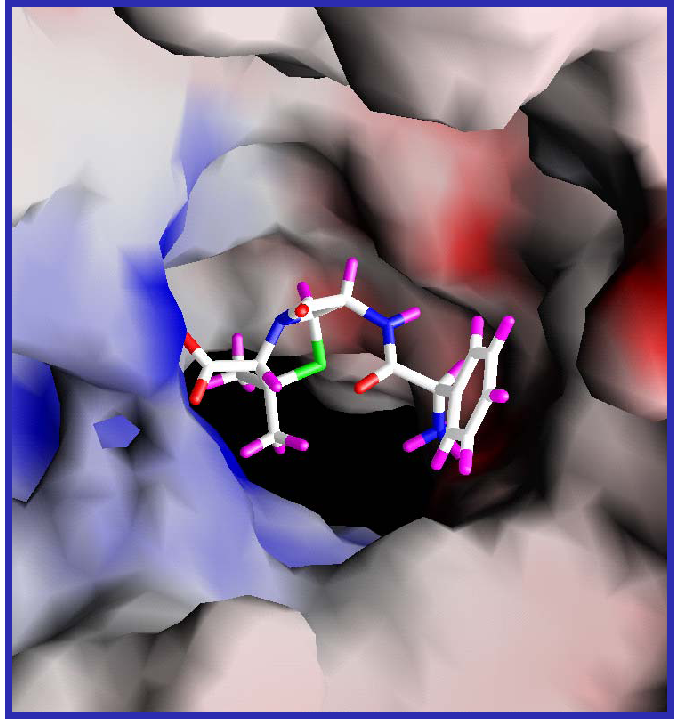
\includegraphics[width=\hsize]{Winterhalter/Winterhalter_fig1.pdf}
    \mycaption{Molecular modelling revealed a binding site for Ampicillin inside an OmpF channel.}
    \label{fig1:Winterhalter}
  \end{center}
\end{figure}

In collaboration with Dr. S.M. Bezrukov (National Institutes of Health, Bethesda,
 USA) we could resolve a single lambda phage binding to its receptor maltoporin.\newline \newline Mathias Winterhalter is also involved in ``Nanocapsules''.
%
% to reference it use ``Figure.~\ref{fig:xxx}''; the numbers will be computed automatically.

% to include a figure, generate a file xxx.pdf and integrate the following lines
%\begin{figure}[ht]
%  \begin{center}
%    \includegraphics[width=6cm]{fig2.pdf}
%    \caption{Typical tracks of ion currents through single trimeric OmpF channels reconstituted into planar lipid membranes at the presence of zwitterionic and anionic penicillins. Membrane bathing solutions contained 1M NaCl (pH 5.0), 5.7 mM of indicated antibiotic, and the applied voltage was -100 mV.  Time resolution was 0.015 msec. (A) Penetrating zwitterionic (ampicillin or amoxicillin) amino penicillins modulate ion current through OmpF.  In the absence of antibiotic (left) the ion current is mainly determined by the geometry and surface properties of the channel pore.  The current is stable; no high-amplitude interruptions are seen.  In the presence of 5.7 mM ampicillin (middle) or amoxicillin (right), one of the three OmpF pores gets spontaneously blocked by a translocating drug molecule.  At high time resolution these blockages are seen as well defined steps to 2/3 of the open channel current and back.  (B) Anionic penicillins do not significantly affect ion current through OmpF.  No interruptions in the current can be seen in the presence of piperacillin (left), azlocillin (middle) or carbenicillin (right).}
%    \label{fig2:Winterhalter}
%  \end{center}
%\end{figure}

\paragraph{Organization}
\begin{enumerate}
\item  We organized a summerschool on Biosensing: Faster smaller, smarter shop at International University
(28.7.-4.8.) with more than 100 participations from 12 countries. A second summerschool on Complex
Materials from June 24th to July 1st. This summerschool included lectures and practical
courses for about 50 participants in the field.
\end{enumerate}



\myparagraph{Collaborations}
%
Bremen Area Collaborations:
\begin{enumerate}
\item {\sl International University Bremen} \\ Prof. J. Fritz \\ Microfluidics for electrophysiology and liposome separation
 \\ Prof. U. Kleinekath�fer \\ Ion and antibiotics transport
through membrane proteins  \\ Prof. S. Springer \\ Injection of
engineered nanocapsules into cells for use as sensors  \\ Prof. M.
Ullrich \\ Multidrug Efflux pumps
\item {\sl Universit�t Bremen, Chemie} \\ Prof. D. Gabel \\ Liposome as carriers
\item {\sl Hochschule Bremen} \\ Prof. V. Hass \\ Process control
\end{enumerate}
National \& International Collaborations:
\begin{enumerate}
\item {\sl University of W�rzburg} \\Prof.  R. Benz \\ Porin
\item {\sl NIH, Bethesda}\\ Dr. S.M. Bezrukov \\ Single molecule transport
\item {\sl MPI Berlin} \\ Prof.  G.B. Sukhorukov \\ Functional
nanocapsules
\item {\sl University of Toulouse} \\ Prof.  D. Fournier \\ Functional
nanocapsules
\item {\sl University of Toulouse}\\ Prof.  P. Faller \\ Microcalorimetry
\item {\sl University of Porto} \\ Prof.  P. Gameiro \\ Antibiotic
translocation
\item {\sl University of Syrakuse} \\ Prof.  L. Movileanu \\ OmpF
characterisation
\item {\sl University of Copenhagen}\\ Prof.  T. Heimburg \\ Lipip phase
transition\end{enumerate}

\paragraph{Grants}
\begin{enumerate}
\item Funded by EU, Training network \emph{Molecular origin of
antibiotic translocation}. This project is performed in
collaboration with N. Fertig (M�nchen), H. Vogel (Lausanne), J.M.
Pages (Marseille), P. Gameiro (Porto), M. Page (Basel), PI M.
Winterhalter.,  (January 2006 - December 2006)

\item Funded by Volkswagen Stiftung,  \emph{Complex Materials:
Cooperative Projects of the Natural, Engineering, and Biosciences:
Nanoengineered polymer capsules: Detection and manipulation for
nanoreactors and controlled delivery.} (I/80 051) in collaboration
with G. B. Sukhorukov (coordinator, MPI Potsdam), A. L. Rogach
(LMU Munich) and W. J. Parak (LMU Munich), (October 2004 -
September 2007)

\end{enumerate}

\paragraph{Other Support Grants}
\begin{enumerate}
\item Volkwagen Stiftung ``Summerschool on Complex Materials'':
\item Eureka 3271 Nano to Bio (PI L. Levy, Nanobiotix, Paris; J.F. Hochepied, Ecole des Mines, Paris)

\item German-french University: Summerschool on Biosening, faster, smaller, smarter.

\item DAAD Exchange program with Porto
\end{enumerate}

\nocite{Winterhalter1,Winterhalter2,Winterhalter3,Winterhalter4,Winterhalter5,Winterhalter6,Winterhalter7,Winterhalter8,Winterhalter9,Winterhalter10,Winterhalter11,Winterhalter12}
